\documentclass{article}
\usepackage[margin=0.75in]{geometry}
\usepackage[utf8]{inputenc}
\usepackage[section]{placeins}
\usepackage{graphicx}
\graphicspath{{./images/}}
\usepackage{float}
\usepackage{listings}
\usepackage{framed}

\title{Naive runtime tests}

\begin{document}
\maketitle
These are the first runtime assessment tests I did, unfortunately not
very sophisticated. I wrote my own basic test driver without warmups
or very many iterations. These tests have since been implemented with
Java MicroBenchmark Harness. One advantage of JMH was that it made sure
not to optimize out ``useless" code. That issue came up here where
\texttt{energyStatCheck()} seemed to have no difference between the Java
side and C side. But that's a false result; the JVM optimized out the return
value, since it wasn't actually being used in the test driver. JMH results
for that test show a significant difference, indicating that returning a
string value to Java from C does incur extra overhead.

\section{Runtime Tests}

\begin{figure}[H]
	\centering
	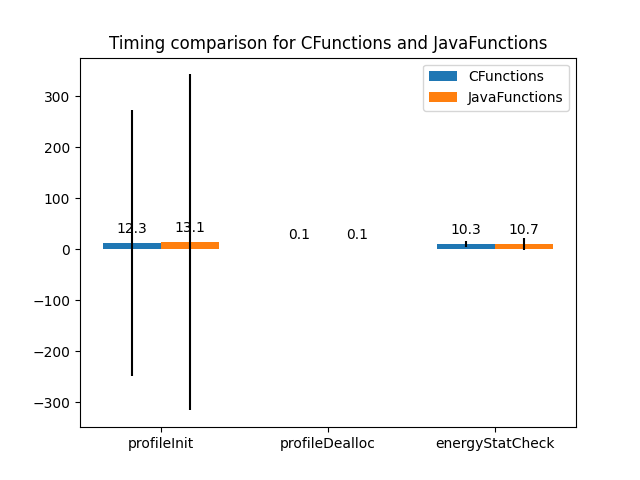
\includegraphics[width=10cm,height=10cm,keepaspectratio]{RuntimeResults_SystemC/CFunctions-JavaFunctions-bar_graph.png}
	\caption{Bar graph comparing Java and C function runtime}
	\label{fig:bar-graph||SystemC}
\end{figure}

\subsection{Java}
    \begin{figure}[H]
   	\centering
    	\includegraphics[width=17cm,height=20cm,keepaspectratio]{RuntimeResults_SystemC/JavaFunctions/runtime-scatters.png}
    	\caption{Scatter plot of Java-Side runtime of native functions for System C}
    	\label{fig:Java-FunctionsSystemC}
    \end{figure}

\subsection{C}

    \begin{figure}[H]
    	\centering
    	\includegraphics[width=17cm,height=20cm,keepaspectratio]{RuntimeResults_SystemC/CFunctions/runtime-scatters.png}
    	\caption{Scatter plot of C-Side runtime of native functions for SystemC}
    	\label{fig:C-Functions|SystemC}
    \end{figure}

\subsection{Time To Read MSRs}

    \begin{figure}[H]
    	\centering
    	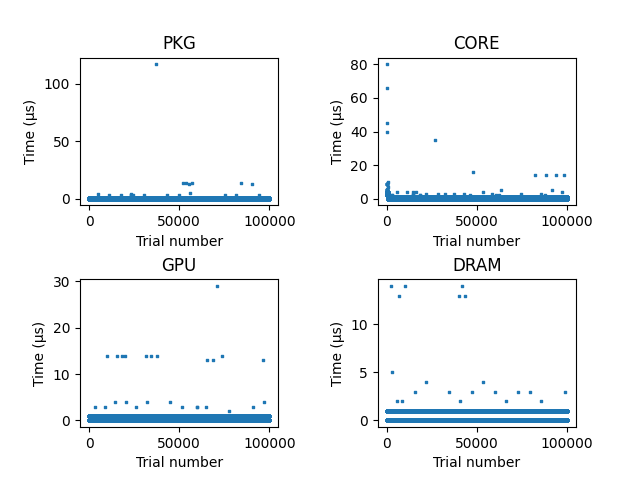
\includegraphics[width=17cm,height=17cm,keepaspectratio]{RuntimeResults_SystemC/PerSocketMSRReadings/Socket1/scatters.png}
    	\caption{Scatter plot of Per-Socket-MSR-Readings runtime for  for SystemC}
    	\label{fig:Per-Socket-MSR-Readings||SystemC}
    \end{figure}

\end{document}